%You can leave alone everything before Line 79.
\documentclass{article}
\usepackage{url,amsfonts, amsmath, amssymb, amsthm,color, enumerate}
% Page layout
\setlength{\textheight}{8.75in}
\setlength{\columnsep}{2.0pc}
\setlength{\textwidth}{6.5in}
\setlength{\topmargin}{0in}
\setlength{\headheight}{0.0in}
\setlength{\headsep}{0.0in}
\setlength{\oddsidemargin}{0in}
\setlength{\evensidemargin}{0in}
\setlength{\parindent}{1pc}
\newcommand{\shortbar}{\begin{center}\rule{5ex}{0.1pt}\end{center}}
%\renewcommand{\baselinestretch}{1.1}
% Macros for course info
\newcommand{\courseNumber}{ME 552}
\newcommand{\courseTitle}{Mechatronics}
\newcommand{\semester}{Fall 2012}
\newcommand{\xxx}[1]{\textcolor{red}{#1}}
% Theorem-like structures are numbered within SECTION units
\theoremstyle{plain}
\newtheorem{theorem}{Theorem}[section]
\newtheorem{lemma}[theorem]{Lemma}
\newtheorem{corollary}[theorem]{Corollary}
\newtheorem{proposition}[theorem]{Proposition}
\newtheorem{statement}[theorem]{Statement}
\newtheorem{conjecture}[theorem]{Conjecture}
\newtheorem{fact}{Fact}
%definition style
\theoremstyle{definition}
\newtheorem{definition}[theorem]{Definition}
\newtheorem{example}{Example}
\newtheorem{problem}[theorem]{Problem}
\newtheorem{exercise}{Exercise}
\newtheorem{algorithm}{Algorithm}
%remark style
\theoremstyle{remark}
\newtheorem{remark}[theorem]{Remark}
\newtheorem{reduction}[theorem]{Reduction}
%\newtheorem{question}[theorem]{Question}
\newtheorem{question}{Question}
%\newtheorem{claim}[theorem]{Claim}
%
% Proof-making commands and environments
\newcommand{\beginproof}{\medskip\noindent{\bf Proof.~}}
\newcommand{\beginproofof}[1]{\medskip\noindent{\bf Proof of #1.~}}
\newcommand{\finishproof}{\hspace{0.2ex}\rule{1ex}{1ex}}
\def\therefore{\boldsymbol{\text{ }
\leavevmode
\lower0.4ex\hbox{$\cdot$}
\kern-.5em\raise0.7ex\hbox{$\cdot$}
\kern-0.55em\lower0.4ex\hbox{$\cdot$}
\thinspace\text{ }}}

\newenvironment{solution}[1]{\medskip\noindent{\bf Problem #1.~}}{\shortbar}

%====header======
\newcommand{\solutions}[4]{
%\renewcommand{\thetheorem}{{#2}.\arabic{theorem}}
\vspace{-2ex}
\begin{center}
{\small  \courseNumber, \courseTitle
\hfill {\Large \bf {#1} }\\
\semester, University of Michigan, Ann Arbor \hfill
{\em Date: #3}}\\
\vspace{-1ex}
\hrulefill\\
\vspace{4ex}
{\LARGE Lab Assignment #2}\\
\vspace{2ex}
\end{center}
\begin{trivlist}
\item \textsc{Team members:\\} {#4}
\end{trivlist}
\noindent
\shortbar
\vspace{3ex}
}
% math macros
\newcommand{\defeq}{\stackrel{\textrm{def}}{=}}
\newcommand{\Prob}{\textrm{Prob}}
%==
\usepackage{graphicx}
\begin{document}
%%%%%%%%%%%%%%%%%%%%%%%%%%%%%%%%%%%%%%%%%%%%%%%%%
%\solutions{Your name}{Problem Set Number}{Date of preparation}{Collaborators}{Prover}{Verifiers}
\solutions{}{2}{\today}{Shiva Ghose, @gshiva\\ John Peterson, @jrpeters\\ Peter Turpel, @pturpel\\ Chan-Rong Lin, @pmelin}
%%%%%%%%%%%%%%%%%%%%%%%%%%%%%%%%%%%%%%%%%%%%%%%%%
%\renewcommand{\theproblem}{\arabic{problem}} 
%%%%%%%%%%%%%%%%%%%%%%%%%%%%%%%%%%%%%%%%%%%%%%%%%
%
% Begin the solution for each problem by
% \begin{solution}{Problem Number} and ends it with \end{solution}
%
% the solution for Problem 

\section*{Question 1}
\subsection*{a.} \xxx{shiva will make block diagram}
\subsection*{b.}
\xxx{The bias voltage helps compensate for the steady state errors in the system. In order to control the position of the ball, we have implemented a lead compensator. The differentiating action of the controller does not account for the steady state errors as the differential of a constant is zero. Thus we manually compensate for the constant errors using the bias voltage. The bias voltage accounts for the constant voltage required to support the weight of the sphere in steady state.  This bias voltage is necessary because because the controller operates on the difference of the measured position and the actual position.  We need this bias to reduce steady state error and generate a strong enough voltage command to the magnet.}
\subsection*{c.}
The photo-transistor passes a current proportional to the amount of light falling on it.  However, our data acquisition card can only measure voltages, rather than currents, so we must convert this current signal into a voltage signal for the card to read by passing this current through a resistor. The resistance of this resistor has been adjusted to make use of the full input voltage range of the DAQ from 0 to 10 volts.\\  We require the voltage following amplifier to avoid loading the sensor circuit when we measure the voltage across this resistor.  This is not strictly necessary when using the DAQ because of its high input impedance, of greater than 10 $G\Omega$, but when we eventually physically implement our controller this may not be the case.  \\

\xxx{Diagram of the of the circuit sensing circuit}\\

\subsection*{d.}
The minimum resistance that can be used in the emitter circuit is dictated by the maximum amount of current that the IR LED can draw, in steady state, without burning out.  \xxx{finish explanation below}
\xxx{finish equations}
\begin{center}
$ \Sigma{V} = 15 - 1.6 - V_0 $
\end{center}

\begin{figure}[hbt]
\begin{center}
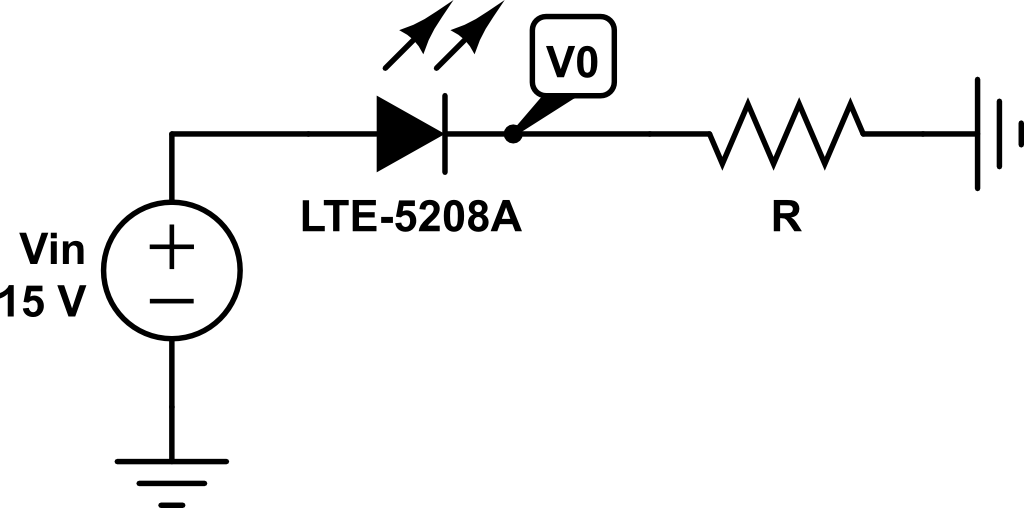
\includegraphics[width = 10cm]{lab2_emitter.png}
\end{center}
\caption{Emitter circuit}
\label{q1_df1}
\end{figure}
A lower resistance should allow the circuit to pass more current which result in a brighter IR beam. This brighter beam will result in a higher signal to noise ratio, because this extra brightness will help to overpower ambient IR sources. It does not effect the full scale range of our detector circuit because this resistance has been tunned to ensure that range between the unblocked beam \xxx{with the magnet present and blocking part of it} and the fully blocked beam is 10 volts. \\  

\subsection*{e.}
It depends on the nature of the failure. \\
If $R_lim$ fails by shorting out then the maximum current is 750 $mA$ \\
$I_{Lim} = \frac{(5000)*(4.75)}{31600\Omega + R_{CL}} $\\
If $R_{Lim}$ is intact and a another component fails, then the maximum current is 510 $mA$. \\
$I_{Lim} = \frac{(5000)*(4.75)}{31.600k\Omega + 14.9k\Omega} =510.64mA$ \\
If the electromagnet somehow became shorted across $+V$ and $-V$, then it would see a potential difference of 30 V.  The coil's internal resistance is 32 $\Omega$ yielding a current of 0.9375 A, and a power dissipated of 28.125 W, which may be enough to cause the coil to overheat.\\
\begin{center}
$I = \frac{V}{R} = \frac{30}{32} = 0.9375 A \hspace{1cm}  P = \frac{V^{2}}{R} = \frac{30^2}{32} = 28.125 W $
\end{center}
If the coil sorted out but remained in series with any of the other components, most of them would be unable to handle the large current draw and rapidly fail.  We would recommend a fuse in series with the coil with 10\% more current rating than our current limit, yielding a ratting of 560 $mA$\\

\subsection*{f.}  We would like the lower limit to be 0 volts, because feeding negative voltage to the magnet would elicit the non-linear behavior of the electromagnet.  In a linear system, we would expect this negative signal to push the sphere away, but in this non-linear system it would attract the sphere.  Limiting the lower range to 0 avoids this non-linearity.  
Our present current limit 510 $mA$.  This current would require an input voltage of 12.07 $V$ into the driver circuit.  Our DAQ is limited to a maximum output of 10 V, and in practice even with the beam unobstructed the system in demands approximately 2.5 V, but with transient effects will demand upwards of $5.5*10^7$ $V$ if the sensor reading steps through its full scale, 0 to 10V range in a single time step. Making it necessary to limit the maximum command voltage to a sensible value.  We choose 5 volts as this does not seem to effect steady state operation and the limit is high enough to allow spikes in the control voltage that the controller wants.

\begin{center}
$V_{command} \approx P * \frac{dV_{sensor}}{dt}  = \frac{0.37 * 5500 * (10 - 0)}{0.001} = 5.5*10^7$
\end{center}

\xxx{Since we are using this voltage to control current, we want to limit the voltage to limit the current to a safe level that can be maintained to not overheat the coil}

\subsection*{g.}
No, the polarity of the electro-magnet does not matter in this application because either pole of the magnet will attract a piece of ferromagnetic material. \xxx{comes down to $i^2$ term}
\xxx{mathematical argument about force being proportional to $i^2$ so current direction doesn't matter} \\
\xxx{need to go through derivation on lecture 234 on slide 20}

\subsection*{h.}
These capacitors buffer the large current requirements of the electromagnet when it turns on. 
$V_i(t) = L\frac{di(t)}{dt}$

\xxx{need picture of nominal response with and without capacitors should see difference}\\
\xxx{graph of supply voltages and see if lack of capacitor is messing them up}\\

\xxx{make note of our use of the flyback diode, want to show that it improves response, so run an experiment and compare transient current response with and without it in place} \\

\xxx{make a note of vdroop on sensor} \\

\end{document}